\errorcontextlines 999999
\PassOptionsToPackage{table}{xcolor}
\PassOptionsToPackage{defernumbers=true}{biblatex}
\documentclass[aspectratio=169,usepdftitle=true,11pt,fleqn,english,c]{beamer}

\usepackage{babel}

\usepackage[%
    sopra-listings={encoding,cpalette,fakeminted,highlights},%
    sopra-tables, color-palettes={addons},%
    lecture-bibliography={biber,style=numeric-comp},%
    util, lithie-boxes={germanenv,koma,overwrite},%
    lithie-task-boxes={cpalette}, lecture-links={patchurl},%
    lecture-registers={disable}% would interfere with beamer
]{lithie-util}

\solLoadLanguage{bash,javascript}
\makeatletter
\sol@list@define@styles{%
  {keywordA: \@declaredcolor{sol@colors@lst@keywordA}\bfseries},%
}
\makeatother

\RestyleAlgo{plain}
\lstset{lineskip=5.5pt}
\lstfs{10}

\DefinePalette{Rekursion}
{Red,rötlich: RGB(93, 46, 70)}
{Blau,bläulich: RGB(22, 105, 122)}
{Lila,lilafarben: RGB(93, 45, 108)}
{Grün,grünlich: RGB(21, 150, 90)}
\SetShadeContrast{51}
\UsePalette{Rekursion}

\usetheme[libs,nofootfade,centerfoot]{dividing-lines}
\SetColorProfile*{paletteA}{paletteB}{paletteC}

\usetikzlibrary{arrows.meta,decorations,tikzmark,matrix,decorations.pathmorphing, decorations.pathreplacing, decorations.shapes}
\def\info#1{\bgroup\scriptsize\textcolor{gray}{(#1)}\egroup}
\SetAllLinkStyle{#1}
\def\fillfont{\def\mdseries@sf{medium}\sffamily}
\colorlet{lgray}{lightgray!48!white}

\usepackage[glows]{tikzpingus}
\usetikzlibrary{decorations.text,graphs}
\hypersetup{colorlinks=false}
\def\rhead#1{\hfill\textcolor{shadeA}{\sbfamily#1}}

\newsavebox\parallellogo
\setbox\parallellogo=\hbox{\tikzpicture[xscale=1.25] % stretch me
\foreach[count=\y from 0] \line in {0,.25,.5,.25,0,.25,.5,.25,0} {
\scope[shift={(\line,-\y)}]
  \foreach\i in {1,3,...,14} {
    \fill (\i,0) rectangle ++(1,1);
    % bars
    \draw[gray,very thick] (\i,0) -- ++(0,1) (\i+1,0) -- ++(0,1);
  }
  \draw[gray,very thick] (0,0) rectangle ++(15,1);
\endscope
}
\endtikzpicture}
% no depth!
\title{\texorpdfstring{\smash{\resizebox*!{\ht\strutbox}{\copy\parallellogo}}~}{}GNU parallel}
\subtitle{Parallelizing and\texorpdfstring{\\}{\space}Distributing programs with the Shell}
\institute{\textsc{ccpdp}, Universität Ulm}

\author[Felix R. \& Florian S.]{Felix Rieg and Florian Sihler}
\email{florian.sihler@uni-ulm.de}

\date{\today}
\outro{Ulm \today}
\license[]{All rights reserved}

\colorlet{codeouthl}{gray!42!white}

\newsavebox\titleimg
\setbox\titleimg=\hbox{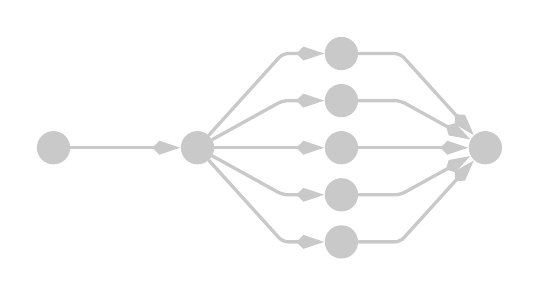
\begin{tikzpicture}[codeouthl]
  \matrix[matrix of nodes,nodes={circle,fill},above right,ampersand replacement=\&,column sep=4em,row sep=.5em] {
           \&        \& |(3a)|~ \&        \\
           \&        \& |(3b)|~ \&        \\
    |(1)|~ \& |(2)|~ \& |(3c)|~ \& |(4)|~ \\
           \&        \& |(3d)|~ \&        \\
           \&        \& |(3e)|~ \&        \\
  };
  % wellp: c\graph[edges={very thick,-Kite}]{(1) -> (2) -> {(3a),(3b),(3c),(3d),(3e)} -> (4)};
  \scope[every path/.append style={draw,very thick,-Kite,rounded corners=2pt,line cap=round}]
  \path(1) -- (2);  \path(2) -- (3c); \path(3c) -- (4);
  \foreach\a in {a,b,d,e} {
    \path (2) -- ([xshift=-1.5em]3\a.west) -- (3\a.west);
    \path (3\a.east) -- ++(1.5em,0) -- (4);
  }
  \endscope
\end{tikzpicture}}
\def\PostTitlepage{\begin{tikzpicture}[overlay,remember picture]
\node[above right=.5cm,xshift=1cm,scale=.875] at(current page.south west) {\copy\titleimg};
\end{tikzpicture}}

\addbibresource{./references.bib}

\makeatletter
\newcommand*\md{\@ifstar{\@md}{\@md{0}}}% with star we can set handout state
\def\@md#1#2{\only<#2|handout:#1>{\llap{\color{shadeA}\textbullet~}}}
\newcommand*\mb[2][0]{\only<#2|handout:#1>{\rlap{\smash{\raisebox{-.66\baselineskip}{\color{shadeA}\textbullet}}}}}
\newcommand*\mh[2][0]{\only<#2|handout:#1>{\color{shadeA}\textbullet}}
\newcommand*\mdl[2][0]{\only<#2|handout:#1>{\llap{\smash{\raisebox{-.5\baselineskip}{\tikz{\fill[shadeA,rounded corners=1pt] (0,-.65mm) rectangle ++(2.15\p@,\baselineskip+.65mm);}}~}}}}
\makeatother


\setcounter{tocdepth}{4}
\newsavebox\pinguA \newsavebox\pinguB \newsavebox\pinguC

\usepackage[link]{qrcode}
% TODO
\outroright{% \smash{\raisebox{1.33cm/2}{
% \qrcode[height=1.33cm]{https://github.com/EagleoutIce/Episode-Recursion}}}\begin{tikzpicture}[remember picture,overlay]
% \node[above left,btdl@color@white,scale=.475] at (current page.south east) {\href{https://github.com/EagleoutIce/Episode-Recursion}{Slides and \LaTeX-sources on GitHub!}};
% \end{tikzpicture}
}

\long\def\commy#1{\smash{\tiny\fboxsep=1pt\fcolorbox{pingu@purple}{pingu@purple!10!white}{\bfseries #1}}}
\long\def\flo#1{\commy{Flo:~#1}}
\long\def\felix#1{\commy{Felix:~#1}}

\usepackage{xspace}
\def\LogoParallel{parallel\xspace}%{para\textit{ll}\/el\xspace}
\makeatletter
\def\sol@minted@setup#1#2#3{\lstset{style=#1,language=#2,lineskip=4pt,#3,escapeinside={/*}{*/}}}
\solsetmintedstyle{plain}% number}

\def\HStrut{\vphantom{\{\}g}}
% we do not nest inside tikzmarknode as this is not possible
\def\Snode#1{\tikzmarknode{#1}\HStrut}
\def\bnode#1#2{\rnode{#1}{\sbasic{#2}}}%
\def\rnode#1#2{\Snode{#1}#2\Snode{#1@}}
\def\CodeFileMarker#1{{\color{gray}\sffamily\fontseries{l}\tiny\llap{\faFileCodeO~\thinspace}#1}}

\def\SetupLstHl{%
\lstcolorlet{highlight}{codeouthl}%
\sol@list@define@styles{%
 {highlight: \@declaredcolor{sol@colors@lst@highlight}\upshape},%
}}

% man spricht ihn Oler Tahng er [http://ole.tange.dk/personen/resume.html]

% git://git.savannah.gnu.org/parallel.git
\begin{document}
\section{Motivation}
% \SidebarCite{book:javase15-std}
\SidebarFakeCite{parallel-tool}
\begin{frame}[c]{Motivation}
% FELIX&FLO
\centering
\onslide<2->{Doing stuff parallel.}\hskip3cm\null\medskip\par
\null\hskip3cm\onslide<3->{With the commandline!}
\end{frame}
\SidebarReset
\section{Background}
\makeatletter % faulheit!
\begin{frame}[c]{Pipes}
\centering
% \begin{layout-imageonly}
\begin{tikzpicture}[,codeouthl,every path/.append style={line cap=round,rounded corners=2pt}]
   \onslide<2->{\node[circle,minimum size=1cm,fill] (@) at(0,0) {};}
   \onslide<3->{\draw[{Kite[scale=.8]}-,very thick](@.west) to[edge node={node[above,black] {\textsc{stdin}}}] ++(-2,0) coordinate (@i);}
   \onslide<4->{\draw[-{Kite[scale=.8]},very thick](@.east) to[edge node={node[above,black] {\textsc{stdout}}}] ++(2,0) coordinate (@O);}
   \onslide<5->{\draw[-{Kite[scale=.8]},very thick](@.north) |- ++(2,.5) node[pos=.75,above,black] {\textsc{stderr}};}
   \onslide<6->{\node[below,darkgray] (wc) at(@.south) {\sbfamily\bbash{wc -l}};}
   \only<7->{
   \scope[xshift=-6cm]
   \onslide<7->{\node[circle,minimum size=1cm,fill] (@) at(0,0) {};
   \draw[{Kite[scale=.8]}-,very thick](@.west) to[edge node={node[above,black] {\textsc{stdin}}}] ++(-2,0) coordinate (@I);
   \draw[-{Kite[scale=.8]},very thick](@.east) to[edge node={node[above,black] {\textsc{stdout}}}] ++(2,0)  coordinate (@o);
   \draw[-{Kite[scale=.8]},very thick](@.north) |- ++(2,.5) node[pos=.75,above,black] {\textsc{stderr}};}
   \onslide<8->{\node[below,darkgray] (cat) at(@.south) {\sbfamily\bbash{cat makefile}};}
   \endscope
   }
   \only<9->{
      \pgfinterruptboundingbox
      \draw[-Kite,very thick,codeouthl!70!white] (@o) -- (@i) coordinate[pos=.5] (@@);
      \path (@@|-wc) node[darkgray,xshift=-1mm] {\sbfamily\T{|}};
      \endpgfinterruptboundingbox
   }
   \only<10->{
      \draw[decorate,decoration={brace,mirror,amplitude=2pt},thick,black,sharp corners] ([yshift=-1.25cm]@I) to[edge node={node[below=2pt] {Producer}}] ([yshift=-1.25cm]@o);
      \draw[decorate,decoration={brace,mirror,amplitude=2pt},thick,black,sharp corners] ([yshift=-1.25cm]@i) to[edge node={node[below=2pt] {Consumer}}] ([yshift=-1.25cm]@O);
   }
   % TODO: next slide, connect them with the pipe symbol
   % TODO: make programs black to read them better
\end{tikzpicture}
% \end{layout-imageonly}
% each program run in the command line has three data streams connected to it:
% \begin{tikzpicture}[@O]
% \scope[shift={(current page.south west)},shift={(\beamer@leftmargin,1cm)}]
% \endscope
% \end{tikzpicture}
\end{frame}

% TODO: example from: https://www.usenix.org/system/files/login/articles/105438-Tange.pdf
\begin{frame}[c]{Pipes\rhead{II}}
\centering\vspace*{.125em}
\begin{layout-imageonly}
\begin{tikzpicture}[,codeouthl,every path/.append style={line cap=round,rounded corners=2pt}]
   \only<-4|handout:0>{\node[circle,minimum size=1cm,fill] (@) at(0,0) {};
   \pgfinterruptboundingbox
   \draw[-{Kite[scale=.8]},very thick](@.north) |- ++(2,.5) node[pos=.75,above,black] {\textsc{stderr}};
   \endpgfinterruptboundingbox
   }
   \only<5->{
      \pgfinterruptboundingbox
      \node[rectangle,minimum width=3cm,minimum height=2cm,very thick,draw] (@) at(0,0) {};
      \draw[-{Kite[scale=.8]},very thick](@.north) |- ++(2,.5) node[pos=.75,above,black] {\textsc{stderr}};
      \endpgfinterruptboundingbox
   }
   \onslide<6->{
      \node[circle,minimum size=1cm,fill] (@sub) at(0,0) {};
      \draw[{Kite[scale=.8]}-,very thick,line cap=rect](@sub.west) -- ++(-1cm+.1mm,0) coordinate (@i);
      \draw[-{Kite[scale=.8]},very thick](@sub.east) -- ++(1,0) coordinate (@O);
      \draw[-{Kite[scale=.8]},very thick](@sub.north) -- ++(0,.5);
      \node[below,darkgray,scale=.8] (wc) at(@sub.south) {\sbfamily\bbash{gzip}};
   }
   % no O1 for xargs: https://www.mankier.com/7/parallel_alternatives#DIFFERENCES_BETWEEN_GNU_Parallel_AND_ALTERNATIVES-DIFFERENCES_BETWEEN_xargs_AND_GNU_Parallel
   \draw[{Kite[scale=.8]}-,very thick](@.west) to[edge node={node[above,black] {\textsc{stdin}}}] ++(-2,0) coordinate (@i);
   \draw[-{Kite[scale=.8]},very thick,line cap=rect](@.east) to[edge node={node[above,black] {\textsc{stdout}}}] ++(2,0) coordinate (@O);
   \onslide<4->{\node[below,darkgray] (wc) at(@.south) {\sbfamily\bbash{xargs gzip}};}
   % NOTE: use --keep! and maybe --recursive for data

   \scope[xshift=-7cm]
   \node[circle,minimum size=1cm,fill] (@) at(0,0) {};
   \draw[{Kite[scale=.8]}-,very thick](@.west) to[edge node={node[above,black] {\textsc{stdin}}}] ++(-2,0) coordinate (@I);
   \draw[-{Kite[scale=.8]},very thick](@.east) to[edge node={node[above,black] {\textsc{stdout}}}] ++(2,0)  coordinate (@o);
   \draw[-{Kite[scale=.8]},very thick](@.north) |- ++(2,.5) node[pos=.75,above,black] {\textsc{stderr}};
   \onslide<2->{\node[below,darkgray] (ls) at(@.south|-wc.north) {\sbfamily\bbash{find . -type f}};}
   \onslide<3->{\node[below=2mm,inner sep=1.5mm,fill=gray!10!white,rounded corners=2pt,text width=3cm,text=black,align=left,font=\ttfamily,scale=.85] at([xshift=1cm]ls.south) {%
      ./Dockerfile\\
      ./run-docker\\
      ./makefile\\
      \vdots
   };}
   % ls hat Probleme, ist hier nur als einfaches Beispiel:
   % https://unix.stackexchange.com/questions/128985/why-not-parse-ls-and-what-to-do-instead
   \endscope
   \draw[-Kite,very thick,codeouthl!70!white] (@o) -- (@i) coordinate[pos=.5] (@@);
   \path (@@|-wc) node[darkgray,xshift=-1mm] {\sbfamily\T{|}};
   % TODO: benchmarks
\end{tikzpicture}
\end{layout-imageonly}
% each program run in the command line has three data streams connected to it:
\end{frame}

\begin{frame}[c]{Pipes\rhead{III}}
   \centering\vspace*{.125em}
\begin{layout-imageonly}
   \begin{tikzpicture}[,codeouthl,every path/.append style={line cap=round,rounded corners=2pt}]
      \onslide<-2|handout:0>{\pgfinterruptboundingbox
      \node[rectangle,minimum width=3cm,minimum height=2cm,very thick,draw] (@) at(0,0) {};
      \endpgfinterruptboundingbox}
      % keeps old @ to avoid jumps
      \onslide<2-|handout:0>{\node[below,darkgray] (wc) at(@.south) {\only<-2|handout:0>{\sbfamily\bbash{parallel gzip}}\only<3->{\phantom{\sbfamily\bbash{parallel gzip}}}};}
      \only<-2|handout:0>{
         \node[circle,minimum size=1cm,fill] (@sub) at(0,0) {};
         \draw[{Kite[scale=.8]}-,very thick,line cap=rect](@sub.west) -- ++(-1cm+.1mm,0) coordinate (@i);
         \draw[-{Kite[scale=.8]},very thick](@sub.east) -- ++(1,0) coordinate (@O);
         \draw[-{Kite[scale=.8]},very thick](@sub.north) -- ++(0,.5);
         \node[below,darkgray,scale=.8] (gz-wc) at(@sub.south) {\sbfamily\bbash{gzip}};
      % TODO: multiples
      }
      \only<3->{
         \pgfinterruptboundingbox
         \node[rectangle,minimum width=3cm,minimum height=5.5cm,very thick,draw] (@) at(0,0) {};
         \endpgfinterruptboundingbox
         \fill (@.west)++(0,.25) arc(90:-90:.25);
         \fill (@.east)++(0,.25) arc(90:270:.25);
         \fill (@.north)++(.25,0) arc(0:-180:.25);

         % hardcode copy-paste love
         \node[circle,minimum size=1cm,fill] (@sub2) at(0,-1.75) {};
         \draw[{Kite[scale=.8]}-,very thick,line cap=rect](@sub2.west) -- ++(-1cm+.1mm+5mm,0) -- ++(-5mm,1.75);
         \draw[-{Kite[scale=.8]},very thick,shorten >=.25cm](@sub2.east) -- ++(1-.5,0) -- ++(.5,1.75);
         \draw[-{Kite[scale=.8]},very thick,codeouthl!60!white,shorten >=.25cm](@sub2.north) to[bend left=8] ++(0,.5+2*1.75);
         \node[below,darkgray,scale=.8] (gz-wc) at(@sub2.south) {\sbfamily\bbash{gzip}};
         \node[circle,minimum size=1cm,fill] (@sub) at(0,0) {};
         \draw[{Kite[scale=.8]}-,very thick,line cap=rect](@sub.west) -- ++(-1cm+.1mm,0) coordinate (@i);
         \draw[-{Kite[scale=.8]},very thick](@sub.east) -- ++(1-.25,0) coordinate (@O);
         \draw[-{Kite[scale=.8]},very thick,codeouthl!60!white,shorten >=.25cm](@sub.north) to[bend right=8] ++(0,.5+1.75);
         \node[below,darkgray,scale=.8] (gz-wc) at(@sub.south) {\sbfamily\bbash{gzip}};
         \node[circle,minimum size=1cm,fill] (@sub1) at(0,1.75) {};
         \draw[{Kite[scale=.8]}-,very thick,line cap=rect](@sub1.west) -- ++(-1cm+.1mm+5mm,0) -- ++(-5mm,-1.75);
         \draw[-{Kite[scale=.8]},very thick,shorten >=.25cm](@sub1.east) -- ++(1-.5,0)  -- ++(.5,-1.75);
         \draw[-{Kite[scale=.8]},very thick](@sub1.north) -- ++(0,.5);
         \node[below,darkgray,scale=.8] (gz-wc) at(@sub1.south) {\sbfamily\bbash{gzip}};
      }
      \draw[{Kite[scale=.8]}-,very thick](@.west) to[edge node={node[above,black] {\textsc{stdin}}}] ++(-2,0) coordinate (@i);
      \draw[-{Kite[scale=.8]},very thick,line cap=rect](@.east) to[edge node={node[above,black] {\textsc{stdout}}}] ++(2,0) coordinate (@O);
      \pgfinterruptboundingbox
      \draw[-{Kite[scale=.8]},very thick](@.north) |- ++(2,.5) node[pos=.75,above,black] {\textsc{stderr}};
      \endpgfinterruptboundingbox

      \onslide<3->{\node[below,darkgray] (pgz) at(@.south) {\sbfamily\bbash{parallel gzip}};}
      % NOTE: use --keep! and maybe --recursive for data

      \scope[xshift=-7cm]
      \node[circle,minimum size=1cm,fill] (@) at(0,0) {};
      \draw[{Kite[scale=.8]}-,very thick](@.west) to[edge node={node[above,black] {\textsc{stdin}}}] ++(-2,0) coordinate (@I);
      \draw[-{Kite[scale=.8]},very thick](@.east) to[edge node={node[above,black] {\textsc{stdout}}}] ++(2,0)  coordinate (@o);
      \draw[-{Kite[scale=.8]},very thick](@.north) |- ++(2,.5) node[pos=.75,above,black] {\textsc{stderr}};
      \node[below,darkgray] (ls) at(@.south|-wc.north) {\sbfamily\bbash{find . -type f}};
      \node[below=2mm,inner sep=1.5mm,fill=gray!10!white,rounded corners=2pt,text width=3cm,text=black,align=left,font=\ttfamily,scale=.85] at([xshift=1cm]ls.south) {%
         ./Dockerfile\\
         ./run-docker\\
         ./makefile\\
         \vdots
      };
      \endscope
      \draw[-Kite,very thick,codeouthl!70!white] (@o) -- (@i) coordinate[pos=.5] (@@);
      \path (@@|-wc) node[darkgray,xshift=-1mm] {\sbfamily\T{|}};

      % TODO: benchmarks
   \end{tikzpicture}
\end{layout-imageonly}
% TODO: übergang pipe animation
% Nicer: https://www.usenix.org/system/files/login/articles/105438-Tange.pdf
\end{frame}
% TODO: nice example clock:
% parallel -k echo {1}'{=3 $_=$_%2?":":" "=}'{2}{3} \
% ::: {0..12} ::: {0..5} ::: {0..9}
% from manual
% TODO: even with grouping, e.g by piping with 'sort' - a stateful operation which operates as "Flaschenhals"
% TODO: auch auf ::: und so eingehen % FLORIAN


\section{GNU \LogoParallel}
\begin{frame}[fragile]{A simple Bank}
\centering\begin{onlyenv}<2-8|handout:1>
\centering\begin{tikzpicture}[codeouthl,xscale=2]
   \scope[K/.style={circle,fill,scale=1.25}]
      {\only<3-4|handout:0>{\color{shadeA}}\node[K] (1) at (0,0) {};
         \onslide<3-4>{\node[gray,below=-.25mm] at(1.south) {\faUser};}
         \onslide<3->{\node[black,above] at(1.north) {Producer};}
      }
      \node[K,codeouthl!60!white] (2) at (1,0) {};
      {\only<5-6|handout:0>{\color{shadeA}}
         \node[K] (3a) at (2,2) {};
         \node[K] (3b) at (2,1) {};
         \node[K] (3c) at (2,0) {};
         \node[K] (3d) at (2,-1) {};
         \node[K] (3e) at (2,-2) {};
         \onslide<5-6>{\foreach \a in {a,b,c,d,e} {\node[gray,below=-.25mm] at(3\a.south) {\faUser};}}
         \onslide<5->{\node[black,above] at(3a.north) {Consumer~1};}
      }
      {\only<7-8|handout:0>{\color{shadeA}}
         \node[K] (4) at (3,0) {};
         \onslide<7->{\node[black,right] (4d) at(4.east) {Consumer~2};}
         \onslide<8->{
            \node[black,below=.5mm,align=left,font=\ttfamily] at(4d.south) {Abby: \kern.8pt-11\\Bert: ~~3\\Carlos: 2\\\vdots};
         }
      }
   \endscope
   \scope[every path/.append style={draw,very thick,-Kite,rounded corners=2pt,line cap=round}]
   \path(1) -- (2) coordinate[pos=.5] (@12);
   \onslide<4->{\node[black,below=.5mm,align=left,font=\ttfamily] at(@12.south) {1 4 3\\1 3 8\\3 2 2\\\vdots};}

   \path[codeouthl!60!white] (2) -- (3c); \path(3c) -- (4);
   \foreach[count=\i]\a in {a,b,d,e} {
      \path[codeouthl!60!white] (2) -- ([xshift=-1.5em]3\a.west) -- (3\a.west);
     \path (3\a.east) -- ++(1.5em,0) coordinate(@) -- (4);
     \onslide<6->{\ifnum\i=1
         \node[black,right=2.75mm,font=\ttfamily,align=left] at(@.east) {\T{Abby -3}\\\T{Bert ~3}\\Abby -8\\\vdots};
      \fi}
   }
   \endscope
\end{tikzpicture}
\end{onlyenv}
\begin{onlyenv}<9-|handout:2->
\begin{tikzpicture}[@O]
\scope[shift={(current page.north east)},shift={(-4cm,-2cm)},codeouthl,xscale=2,K/.style={circle,fill,scale=1.25},scale=.5,every ndoe/.append style={transform shape}]
      {\only<10-13|handout:2>{\color{shadeA}} \node[K] (1) at (0,0) {};}
      \node[K,codeouthl!60!white] (2) at (1,0) {};
      {\only<14-17|handout:3>{\color{shadeA}}
         \node[K] (3a) at (2,2) {};
         \node[K] (3b) at (2,1) {};
         \node[K] (3c) at (2,0) {};
         \node[K] (3d) at (2,-1) {};
         \node[K] (3e) at (2,-2) {};
      }
      {\only<18-20|handout:4>{\color{shadeA}}
         \node[K] (4) at (3,0) {};
      }

      \scope[every path/.append style={draw,very thick,-{Kite[scale=.8]},rounded corners=2pt,line cap=round}]
   \path(1) -- (2) coordinate[pos=.5] (@12);

   \path[codeouthl!60!white] (2) -- (3c); \path(3c) -- (4);
   \foreach[count=\i]\a in {a,b,d,e} {
      \path[codeouthl!60!white] (2) -- ([xshift=-1.5em]3\a.west) -- (3\a.west);
       \path (3\a.east) -- ++(1.5em,0) coordinate(@) -- (4);
   }
   \endscope
\endscope
\end{tikzpicture}
\end{onlyenv}
\begin{onlyenv}<10-|handout:2->
\begin{layout-imageonly}
\begin{onlyenv}<10-13|handout:2>
\begin{tikzpicture}[@O]
   \onslide<11->{\hlbehindcodeunder{n}{@n>}
      \draw[T,-Kite] (@n>_up) to[bend left] ++(.5,.35) node[right] {number of transactions};
   }
   \onslide<12->{\hlbehindcodeunder{names}{@names>}
      \draw[T,-Kite] (@names>_up) to[bend left] ++(.5,.35) node[right] {known account names};
   }

   \onslide<13->{\hlbehindcodeunder{value}{@value>}
      \node[T,below] at (@value>_down) {value};
   }
\end{tikzpicture}
\begin{minted}{java}
/*\CodeFileMarker{Producer.java}*/
final var rand = new Random();

for (int i = 0; i < /*\Snode{n}*/n/*\Snode{n@}*/; i++) {
   int from = rand.nextInt(/*\Snode{names}*/NAMES/*\Snode{names@}*/.length);
   int to = rand.nextInt(NAMES.length);
   System.out.format("%d %d %d%n", from, to, /*\Snode{value}*/rand.nextInt(100) * 10/*\Snode{value@}*/);
}
\end{minted}
% TODO: highlight n as number, names for constants and value
\end{onlyenv}
\begin{onlyenv}<14-17|handout:3>
\begin{tikzpicture}[@O]
   \onslide<15->{
      \hlbehindcodeunder{from}{@from>}
      \draw[T,-Kite] (@from>_up) to[bend left] ++(.5,.35) node[right] {0};
   }
   \onslide<16->{
      \hlbehindcodeunder{to}{@to>}
      \draw[T,-Kite] (@to>_up) to[bend left] ++(.5,.35) node[right] {1};
   }
   \onslide<17->{
      \hlbehindcodeunder{value}{@value>}
      \draw[T,-Kite] (@value>_up) to[bend left] ++(.5,.35) node[right] {2};
   }
\end{tikzpicture}
\begin{minted}{java}
/*\CodeFileMarker{Consumer.java}*/
final var scanner = new Scanner(System.in);
while (scanner.hasNextLine()) {
   String[] s = scanner.nextLine().split(" ");/*\vspace{\medskipamount+1mm}*/
   String from = NAMES[Integer.parseInt(s[/*\Snode{from}*/FROM/*\Snode{from@}*/])];
   System.out.printf("%s -%d%n", from, Integer.parseInt(s[/*\Snode{value}*/VALUE/*\Snode{value@}*/]));/*\vspace{\medskipamount+1mm}*/
   String to = NAMES[Integer.parseInt(s[/*\Snode{to}*/TO/*\Snode{to@}*/])];
   System.out.printf("%s %d%n", to, Integer.parseInt(s[VALUE]));
}
scanner.close();
\end{minted}
\end{onlyenv}
\begin{onlyenv}<18-20|handout:4>
\begin{tikzpicture}[@O]
   \onslide<19->{
      \hlbehindcodeunder{getOrDefault}{@getOrDefault>}
      \draw[T,-Kite] (@getOrDefault>_up) to[bend left] ++(.5,.35) node[right] {Arbitrary initialization};
   }
   \onslide<20->{
      \hlbehindcodeunder{accounts}{@accounts>}
      \draw[T,-Kite] (@accounts>_up) to[bend left] ++(.5,.35) node[right] {\T{AbstractMap.toString()}};
   }
\end{tikzpicture}
\begin{minted}{java}
/*\CodeFileMarker{Accountant.java}*/
final var scanner = new Scanner(System.in);
final var accounts = new HashMap<String, Integer>();
while (scanner.hasNextLine()) {
   String[] trans = scanner.nextLine().split(" ");

   final var old = accounts./*\Snode{getOrDefault}*/getOrDefault(trans[0], 0)/*\Snode{getOrDefault@}*/;
   accounts.put(trans[0], old + Integer.parseInt(trans[1]));
}
scanner.close();
System.out.println(/*\Snode{accounts}*/accounts/*\Snode{accounts@}*/);
\end{minted}
\end{onlyenv}
\end{layout-imageonly}
\end{onlyenv}
\end{frame}

% \subsection{The Running-Example}
{
\lstset{add to literate={\\}{{{\color{codeouthl}{\textbackslash}}}}1}
\def\K#1{\begin{colormixin}{30!black}#1\end{colormixin}}% i dunno, semes to look nice
\newcommand<>\M{\only#1{\color{gray}}}
\newcommand<>\MM[1]{\colorlet{@mixn}{black}\only#2{\colorlet{@mixn}{gray}}\begin{colormixin}{0!@mixn}#1\end{colormixin}}% i dunno, semes to look nice
\def\Q{\only<7->}
\def\Y{\only<12->}
\begin{frame}[fragile,t]{Running the Example} % top for second table?
\centering\vspace*{2em}% top buffer
\SetupLstHl
\begin{onlyenv}<2-8|handout:1>
\begin{minted}{bash}
/*\onslide<3->*/java -jar producer.jar 1000000/*\onslide<4->*/\
	| java -jar consumer.jar/*\onslide<5->*/\
	| java -jar accountant.jar/*\onslide<1->*/
\end{minted}
\end{onlyenv}
% TODO: did it in a makefile so that we see this statement as well (otherwise the host shell would do that)
% ❯ make run-no-parallel& ; sleep 1; ps -o pid,ppid,cpuid,cmd > run.data
% ❯ make run& ; sleep 1; ps -o pid,ppid,cpuid,cmd > run2.data
% C is lastcpu | cpuid
% lwp light weight process (thread)
% PSR is currently assigned processor
% ps -F
\begin{onlyenv}<9|handout:0>
\begin{minted}{bash}
&ihl&java -jar producer.jar 1000000\&ihl&
&ihl&	| java -jar consumer.jar&ihl&
&ihl&	| java -jar accountant.jar&ihl&/*\onslide<3->*/
\end{minted}
\end{onlyenv}
\begin{onlyenv}<10-|handout:2>
\begin{minted}{bash}
&ihl&java -jar producer.jar 1000000\&ihl&
&ihl&	| &ihl&parallel --pipe &ihl&java -jar consumer.jar\&ihl&
&ihl&	| java -jar accountant.jar&ihl&/*\onslide<3->*/
\end{minted}
% TODO: different colors? for ppid -> pid
\end{onlyenv}
\begin{tikzpicture}[@O,outer sep=0pt,inner sep=0pt]
\onslide<11-|handout:2>{\node[above right,xshift=\beamer@leftmargin,yshift=1cm,font=\tiny\ttfamily,text width=14cm] (@) at(current page.south west) {\begin{tabular}{rrrl}
      {pid} & {ppid} & {cpuid} & {cmd} \\ % {lwp} & \rlap{\quad\ldots}
\midrule
  38279 & \M<13->38276 &  \M<13->3 & \MM<13->{\bbash{/bin/bash -c java -jar producer.jar 1000000 | parallel --pipe java -jar consumer.jar | java -jar a:ldots:}}\kern-3pt\\
  \Y{\M<13->38280} & \Y{38279} &  \Y{6} & \Y{\K{\bbash{java -jar producer.jar 1000000}}} \\
  \Y{38281} & \Y{38279} & \Y{15} & \Y{\K{\bbash{perl /usr/bin/parallel --pipe java -jar consumer.jar}}} \\
  \Y{\M<13->38282} & \Y{38279} &  \Y{5} & \Y{\K{\bbash{java -jar accountant.jar}}} \\ % \smallskip\\
  \Y{38344} & \Y{38281} & \Y{10} & \Y{\K{\bbash{perl -e if(sysread(STDIN,\$buf,1))\{open(\$fh }}\textcolor{gray}{\,[\ldots]\!}\K{\} \bbash{/usr/bin/bash -c java -jar consumer.jar}}} \\
  \Y{\M<13->38345} & \Y{38281} &   \Y{\M<13->4} & \MM<13->{\Y{\K{\bbash{perl -e if(sysread(STDIN,\$buf,1))\{open(\$fh }}\textcolor{gray}{\,[\ldots]\!}\K{\} \bbash{/usr/bin/bash -c java -jar consumer.jar}}}} \\
  \Q{\color{gray}\ldots} & \Q{\color{gray}\ldots} & \Q{\color{gray}\ldots} & \Q{\color{gray}\ldots} \\
  \Y{\M<13->38363} & \Y{38281} &  \Y{\M<13->10} & \MM<13->{\Y{\K{\bbash{perl -e if(sysread(STDIN,\$buf,1))\{open(\$fh }}\textcolor{gray}{\,[\ldots]\!}\K{\} \bbash{/usr/bin/bash -c java -jar consumer.jar}}}} \\
  \Y{\M<13->38383}  & \Y{38281} &   \Y{\M<13->4} & \Y{\MM<13->{\bbash{perl /usr/bin/parallel --pipe java -jar consumer.jar}}} \\
  \Y{\M<13->38384}  & \Y{38344} &  \Y{2} & \Y{\K{\bbash{java -jar consumer.jar}}} \\
  \Y{\M<13->38438}  & \Y{\M<13->38136} &  \Y{\M<13->12} & \Y{\MM<13->{\bbash{ps -o pid,ppid,cpuid,cmd}}}
   \end{tabular}};}

   % below right for same position! so it does not jump
   \onslide<6-10|handout:1>{\node[below right,font=\tiny\ttfamily,text width=14cm] (@2) at(@.north west) {\begin{tabular}{rrrl}
         {pid} & {ppid} & {cpuid} & {cmd} \\ % {lwp} & \rlap{\quad\ldots}
   \midrule
   25621 & \M<8->25618 &  \M<8->7 &\rlap{\MM<8->{\bbash{/bin/bash -c java -jar producer.jar 1000000 | java -jar consumer.jar | java -jar accountant.jar}}}% align lap:
   \phantom{\bbash{/bin/bash -c java -jar producer.jar 1000000 | parallel --pipe java -jar consumer.jar | java -jar a:ldots:}\kern-3pt}\\
   \Q{\M<8->25622} & \Q{25621}  &  \Q{2} & \Q{\K{\bbash{java -jar producer.jar 1000000}}} \\
   \Q{\M<8->25623} & \Q{25621}  &  \Q{ 14} & \Q{\K{\bbash{java -jar consumer.jar}}} \\
   \Q{\M<8->25624} & \Q{25621}  &  \Q{ 13} & \Q{\K{\bbash{java -jar accountant.jar}}} \\
   \Q{\M<8->25738} & \Q{\M<8->5113} &  \Q{\M<8->9} & \Q{\MM<8->{\bbash{ps -o pid,ppid,cpuid,cmd}}}
      \end{tabular}};
   }
   \only<0|handout:1>{% TODO: make comment in presentation manually?
      % tikzmark is problematic due to nested tikz and me being lzy
      \draw[-Kite,T] ([xshift=1.5cm,yshift=-.75cm]@2.north) to[bend right] ++(.4,-.4) node[below right,xshift=.5ex,align=left,yshift=.25\baselineskip] {Ran from within a makefile\\(directly done by shell otherwise)};
      \draw[-Kite,T] ([xshift=-2.5cm,yshift=-1.75cm]@2.north) to[bend right] ++(.4,-.4) node[below right,xshift=.5ex,align=left,yshift=.25\baselineskip] {Produces (a superset of) this table};
   }
   \only<0|handout:2>{%
      % tikzmark is problematic due to nested tikz and me being lzy
      \draw[-Kite,T] ([xshift=-1cm,yshift=-2.75cm]@2.north) to[out=0,in=180] ++(.65,-.125) node[below right,xshift=.5ex,align=left,yshift=.2\baselineskip,scale=.8] {Used for generic splitting magic\\(e.g., not done with \bbash{--roundrobin})};
   }
\end{tikzpicture}
% TODO: show roundrobin much simpler only java-jar etc-
%    grafik und Code
% wann sinnvoll usw.
% bank beispiel mit java  %  FELIX
\begin{tikzpicture}[@O]
\scope[shift={(current page.north east)},shift={(-4cm,-2cm)},codeouthl,xscale=2,K/.style={circle,fill,scale=1.25},scale=.5,every ndoe/.append style={transform shape}]
      \only<2-9|handout:1>{{\only<3|handout:0>{\color{shadeA}}\node[K] (1) at (0,0) {};}
      {\only<4|handout:0>{\color{shadeA}}\node[K] (2) at (1,0) {};}
      {\only<5|handout:0>{\color{shadeA}}\node[K] (3c) at (2,0) {};}

      \scope[every path/.append style={draw,very thick,-{Kite[scale=.8]},rounded corners=2pt,line cap=round}]
        \path(1) -- (2) coordinate[pos=.5] (@12);
        \path (2) -- (3c);
   \endscope}
   \only<10-|handout:2>{
      \node[K] (1) at (0,0) {};
      \node[K,codeouthl!60!white] (2) at (1,0) {};
      \node[K] (3a) at (2,2) {};
      \node[K] (3b) at (2,1) {};
      \node[K] (3c) at (2,0) {};
      \node[K] (3d) at (2,-1) {};
      \node[K] (3e) at (2,-2) {};
      \node[K] (4) at (3,0) {};

      \scope[every path/.append style={draw,very thick,-{Kite[scale=.8]},rounded corners=2pt,line cap=round}]
   \path(1) -- (2) coordinate[pos=.5] (@12);

   \path[codeouthl!60!white] (2) -- (3c); \path(3c) -- (4);
   \foreach[count=\i]\a in {a,b,d,e} {
      \path[codeouthl!60!white] (2) -- ([xshift=-1.5em]3\a.west) -- (3\a.west);
       \path (3\a.east) -- ++(1.5em,0) coordinate(@) -- (4);
   }
   \endscope
   }
\endscope
\end{tikzpicture}
% TODO: somewhat like a sleepy consumer 1? so that we can see, how parallel does work
\end{frame}
}

\subsection{History}
\SidebarCite{Tange2011a}
\SidebarFakeCite{gnuHistoryParallel}
\begin{frame}{History}
   \begin{itemize}[<+(1)->]
      \itemsep10pt
      \item Originally two tools: xxargs and \LogoParallel. \begin{itemize}
         \itemsep5pt
         \item Parallel was originally a wrapper that generated a makefile and used \bbash{make -j} to do the parallelization
         \item xxargs and \LogoParallel got merged into parallel
         \item Two objectives: \begin{itemize}
            \item replace xargs % whitespace problems
            \item run commands in parallel
         \end{itemize}
      \end{itemize}
      \item In 2010, \LogoParallel was adopted as an official GNU tool, named GNU \LogoParallel.
   \end{itemize}
   % Single-file to work easily, perl because seems to be widespread, problem: overhead (--tag option+, https://www.gnu.org/software/parallel/parallel_design.pdf)
\end{frame}
\SidebarReset

\subsection{Distribution}
{
\lstset{add to literate={\$SERVER}{{{\color{gray}\textdollar SERVER}}}7 {\$SERVER1}{{{\color{gray}\textdollar SERVER1}}}7 {\\}{{{\color{codeouthl}{\textbackslash}}}}1}
\SidebarRaw{\link{https://www.gnu.org/software/parallel/parallel\_tutorial.html\#transferring-files}{{\faExternalLink}~parallel tutorial~[06/30/22]}}
\begin{frame}[fragile]{Distributed}
\begin{itemize}[<+(1)->]
   \itemsep6pt
   % \item \flo{Felix wo hast du die Beispiele her? Quellen!}
   \item GNU \LogoParallel can run jobs on remote servers \begin{itemize}
      \item It uses ssh to communicate with the remote machines
      \begin{minted}{bash}
parallel -S $SERVER echo running on ::: $SERVER
      \end{minted}
   \end{itemize}
   \item Transfer Files using rsync:
\begin{itemize}
   \item Long version:
   \begin{minted}[deletekeywords={transferfile}]{bash}
parallel -S $SERVER /*\T{-}*//*\T{-}*//*\T{return}*/ {}.out --transferfile\
   {} --cleanup cat {} "/*\T{\solGet{literals}{>}}*/"{}.out ::: input_file
   \end{minted}
   \item Shorthands:
\begin{minted}[deletekeywords={transferfile}]{bash}
parallel -S $SERVER /*\T{-}*//*\T{-}*//*\T{trc}*/ {}.out cat {} "/*\T{\solGet{literals}{>}}*/"{}.out
   ::: input_file
\end{minted}
\end{itemize}
% \item TODO: beautiful shortant
\end{itemize}
   % erweiterungen wei verteilt mehrere Systeme % FELIX (-ssh oder so)
\end{frame}
\SidebarReset

\SidebarRaw{\link{https://www.gnu.org/software/parallel/parallel\_tutorial.html\#avoid-overloading-sshd}{{\faExternalLink}~parallel tutorial~[06/30/22]}}
\begin{frame}[fragile]{Useful Flags}
\begin{itemize}[<+(1)->]
   \itemsep3pt
   \item Prevent \T{sshd} overloading:\pause
\begin{minted}{bash}
parallel -S $SERVER /*\T{-}*//*\T{-}*//*\T{sshdelay}*/ 0.2 echo ::: 1 2 3
\end{minted}
   \item Multiplex connections with \bbash{--controlmaster}
   \item Transfer Files using rsync: \begin{itemize}
      \item \bbash{--basefile}, copy this file to each sshlogin % note: --cleanup
      \item \bbash{--workdir}, change from login directory
      \item \bbash{--onall}, run job on all sshlogins % only mention: /\bbash{--nonall},
      % \item \bbash{--tag} not just for sshlogin
   \end{itemize}
\end{itemize}
% grafik und Code
\end{frame}
\SidebarReset

\subsection{Other Languages}
\begin{frame}[fragile]{Other Languages}
   %Grafik und Code
   \begin{minted}{javascript}
      let accMap = new Map<String, number>();

      const handleLine = (input: String) => {
         const s = input.split(" ");
         if (!accMap.has(s[0])) accMap.set(s[0], 0);
         accMap.set(s[0], accMap.get(s[0])! + +s[1]);
      };

      readline.on("line", handleLine);

   \end{minted}
   \begin{minted}{bash}
      java -jar producer.jar 1000000 | parallel --pipe java -jar consumer.jar | yarn --silent start
      #java -jar producer.jar 1000000 | parallel --pipe java -jar consumer.jar | java -jar accountant.jar
   \end{minted}
   % verschiedene Sprache % FELIX
   % TODO: timeout option?
\end{frame}
\subsection{Data Encoding}
\begin{frame}{Data Encoding}
      Code Json, vs. yaml, vs...
   % objekte % FLORIAN (gson und so)
\end{frame}
}

\subsection{Recap} % maybe not as separate bot in the bottom?
\begin{frame}{Recap}
   \begin{itemize}[<+(1)->]
      \itemsep12pt
      \item Producer-Consumer
      \item stream-based communication \begin{itemize}
         \item cf. Javas functional streams
         \item serialization and deserialization % TODO: talk about advantages and disadvantages
         \item decoupled programs (e.g., no shared memory)
      \end{itemize}
      \item TODO: distribution @Felix (chapter F) stream based stuff
      \item lock-free etc because producer-consumer
      \item TODO: other stuff?
   \end{itemize}
\end{frame}

\section{Inner Workings}
% TOOD: siebar note for bash only https://devdocs.io/bash/pipelines | https://www.gnu.org/software/bash/manual/bash.pdf
\begin{frame}{About pipes}
\begin{itemize}
   \item Execute each program in own subshell
   \item TODO: not sequential: \url{https://stackoverflow.com/a/32946581} os we execute al steps in parallel for free (producer-consumer) % TODO: \url{https://pubs.opengroup.org/onlinepubs/009695399/utilities/xcu_chap02.html\#tag_02_09_02}
   \item TODO: talk about redirection and sockets?
   \item load balacning \url{https://stackoverflow.com/questions/14039403/gnu-parallel-load-balancing}
   \item how does bash sync it?
   \item Parallel --pipe max out at 1Gbs in 100Mbs out
   \item TODO: --roundrobin etc -L for multiple lines
\end{itemize}
% Semaphor => kann als solche verwendet werden
% Semaphor, Rechner Sockets, % FLO
% parallel nutzt die host-shell aus (deisgn: which shell to use, p11)
\end{frame}
\begin{frame}
 TODO: SPREADING BLOCKS OF DATA
 in \url{https://www.gnu.org/software/parallel/parallel.pdf}
 \$Global::JobQueue
 TODO: groupby
 %  synchinc
\end{frame}

\section{Outlook?}
\begin{frame}{Look Out!}
% FELIX&FLO
% praktische Anwendungen
% optionen die wir nicht vorstellen
% gibt es eine geplante Weiterentwicklung? <- ne
% Alternativen: https://www.gnu.org/software/parallel/parallel_alternatives.pdf
% xargs hat -P, makefiles etc.
% -pipe vs pipepart, disk buffering
% sql support --sql-master etc.
% table support
% shebang
\end{frame}

\end{document}